\documentclass[12pt,onecolumn,draftclsnofoot]{IEEEtran}
\usepackage[a4paper,margin=1in]{geometry}
\usepackage{times,graphicx,amsmath,booktabs,cite,url}
\usepackage[ruled,linesnumbered]{algorithm2e}
% Additional packages (figures are drawn in TikZ/PGFPlots, so no screenshots are used)
\usepackage{amssymb,array,multirow}
\usepackage{tikz}
\usetikzlibrary{positioning,arrows.meta,fit,calc}
\usepackage{pgfplots}
\pgfplotsset{compat=1.18}
% Shrink a table to the text width only if it is wider than the page
\newcommand{\fitwidth}[1]{\resizebox{\ifdim\width>\textwidth\textwidth\else\width\fi}{!}{#1}}

\begin{document}

\title{Retrieval-Augmented LLM Agents versus Static Analysis for Technical Debt Prioritisation: A Time-Split Evaluation}

\author{Group 11 (CSE2): Sahil Mahadev Mane (230545), Asad Ahmad (230516), Ayush Singh (230556), Naveen Singh/Kiran Khatter\\
School of Engineering \& Technology, BML Munjal University}

\maketitle

\begin{abstract}
We have built an open source Python pipeline to prioritize technical debt items for refactoring. The pipeline first runs four static code analysis tools on the code under study. It then retrieves the function-level history of the code under study, as well as a call graph of the code under study. It then uses the retrieved code, the history, and the call graph as input to a Retrieval-Augmented Generation (RAG) system to rank each candidate function and generate possible refactorings for it. The generated refactorings are then applied on separate branches of the code under study, and are only accepted if all old tests still pass, the complexity of the code decreases, and the code does not contain any new lint or duplication issues. We use a snapshot of the Requests library taken before 1 January 2024 as input to our experiments, and evaluate the generated rankings against the bug-fix and change commits that were made after that date. On 71 candidate functions, a local 1.7-billion-parameter model reached a Spearman correlation of 0.139 with future changes and a defect ROC-AUC of 0.494, below raw cyclomatic complexity (0.507) and a transparent context heuristic (AUC 0.912); the gap to complexity was significant ($\Delta\rho=-0.369$, 95\% CI $[-0.637,-0.070]$). Larger GPT-OSS models on a 30-item pilot ranked better but still did not beat complexity, and none of five LLM refactorings passed the gate. The study shows that history-aware heuristics are a strong, cheap baseline that LLM prioritisers must beat before they are trusted.
\end{abstract}

\begin{IEEEkeywords}
Large language models, mining software repositories, refactoring, retrieval-augmented generation, technical debt prioritisation.
\end{IEEEkeywords}

\noindent\textbf{Overleaf Project Link:} \url{https://www.overleaf.com/project/REPLACE-WITH-PROJECT-ID}

\section{Introduction}

Technical debt refers to the added work programmers have to do later on as a result of taking code shortcuts which increase the effort and difficulty in changing the code \cite{cunningham1992}. Research has been conducted on various aspects of technical debt including identification and measurement of debt, and ways to repay it \cite{kruchten2012,li2015}. In most cases the first step to repaying technical debt is use of a static analyzer. Other tools to compute cyclomatic complexity of a program, or maintainability indices, can be easily added to a company's continuous integration process \cite{hilton2016}. Recently, large language models have come into use to identify inefficiencies in computer code and recommend refactorings \cite{hou2024}.

Repaying debt is harder than finding debt. For example, running four analysers on the mature and well-tested Requests HTTP library (5,400 lines of code) results in 500 findings, and 84 functions have at least one problem. A developer team cannot refactor all of these. But the analysers provide no criteria for prioritizing functions beyond a simple threshold for each analyzer. For example, two functions with the same complexity may have completely different risks: one function is called from everywhere in the code and is modified every month, the other function is stable code that is never modified. Thus, a good prioritiser would also need repository context such as the change history of a function, its callers, test coverage, etc. in addition to the code metrics.

There are existing approaches that address parts of the problem described in this paper. Many existing identification techniques are listed in mapping studies but few of them are validated against outcomes in prioritisation \cite{li2015,alves2016}. Defect-prediction research focuses on using process metrics such as code churn to predict faults \cite{nagappan2005,hassan2009,kamei2013}. These are used to predict the occurrence of defects, not to prioritize debt to be repaid. The evaluation of LLM tools for code review and refactoring mostly measures the generated code for compilation errors and for tests to pass \cite{shirafuji2023,jimenez2024}. We are not aware of any studies that evaluate how well LLM generated priorities for code maintenance match later maintenance effort. Also, when using an LLM to rank debt in a public repository, there is the risk of prompt leakage, i.e.\ the prompt contains information from after the decision date, or the evaluation silently uses the same history as the input.

This paper asks two research questions.
\begin{itemize}
\item \textbf{RQ1:} Does an LLM agent chain given static metrics, repository context and RAG-retrieved similar items rank technical debt closer to post-cutoff bug fixes and changes than static analysis alone and a non-LLM context heuristic?
\item \textbf{RQ2:} Can the same agents produce refactorings that pass an automated CI gate (no new test failures, lower complexity, no new lint or duplication findings), and which parts of the pipeline account for the observed ranking quality?
\end{itemize}

Our contributions are as follows.
\begin{itemize}
\item An open-source pipeline that combines static analysis tools, function-level Git history, a call graph, RAG-retrieved similar code snippets with ChromaDB and a three-agent LLM chain, and validates the generated refactorings with a CI gate on isolated branches.
\item A leakage-free, time-split evaluation scenario in which all inputs are taken from a snapshot of the repository before a cutoff date and the ground truth is taken from commits after that cutoff date.
\item We compare the LLM ranking with four non-LLM baselines on 71 functions of the Requests library and report bootstrap uncertainty for each of the results. We also perform a Git-history ablation, a retrieved-context ablation, and a model-size comparison.
\item We present five end-to-end LLM refactoring attempts and report on the runtime cost of each pipeline stage on repositories up to 24.75 thousand lines.
\end{itemize}

Section~\ref{sec:related} reviews related work, Section~\ref{sec:background} defines the problem, Section~\ref{sec:method} describes the pipeline, Section~\ref{sec:setup} gives the experimental setup, Section~\ref{sec:results} reports results, and Sections~\ref{sec:discussion} and~\ref{sec:conclusion} discuss the findings and conclude.

\section{Related Work}
\label{sec:related}

\subsection{Identifying and Prioritising Technical Debt}

The technical debt literature is mapped by Li et al. in order to assess the current state of the art on technical debt identification, measurement, prioritization and repayment. They find that most of the work on technical debt has focused on its identification and measurement, with only limited work on its prioritization and repayment, and with even less work being validated empirically \cite{li2015}. Alves et al. also reach similar conclusions about the state of the art in technical debt, and find that many of the techniques for identifying technical debt rely on code smells and on metric thresholds \cite{alves2016}. In addition, Potdar and Shihab found that developers admit debt in comments within source code, and thus started work on the topic of self-admitted technical debt \cite{potdar2014}. However, the comments only describe the debt that developers choose to record. The Requests snapshot that we use contains very few comments that admit to debt. Tufano et al. studied the history of code smells, and found that most of the smelly code is smelly from the point that it was written, and does not decay over time \cite{tufano2015}. Therefore, we can expect that metrics that are measured at a single point in time carry real signal.

Industrial tools such as SonarQube attach a remediation cost to each rule violation. Lenarduzzi et al. released a dataset of SonarQube results, issues and commits for Apache Java projects \cite{lenarduzzi2019tdd} and later tested whether SonarQube rules are associated with fault-inducing commits, finding that only a small part of them are \cite{lenarduzzi2020sonar}. Tsoukalas et al. used SonarQube time series to forecast how debt will grow \cite{tsoukalas2020}. These studies show that static findings and debt are related but that a raw count of findings is a weak guide to where future effort will go. They also stay within static analysis and do not use language understanding to weigh one finding against another.

\subsection{Process Metrics and Defect Prediction}

A large amount of work has been done on defect prediction based on version history. Nagappan and Ball found that relative code churn can predict the defect density of a large commercial system \cite{nagappan2005}. Hassan used the entropy of changes to predict faults \cite{hassan2009}. Kamei et al. predicted defect-inducing changes at the commit level across 11 projects \cite{kamei2013}. \'{S}liwerski et al. linked bug-fix commits to the changes that caused them by mining commit messages \cite{sliwerski2005}. This work motivates the use of context features for defect prediction and provides a fair baseline for evaluating the performance of LLMs for maintenance tasks.

\subsection{LLMs and Agents for Code Maintenance}

Hou et al. provide a systematic review of the literature on LLMs in software engineering \cite{hou2024}. They find that most of the evaluations of LLMs in software engineering are on code generation benchmarks and that maintenance tasks are less studied. SWE-bench showed that resolving real GitHub issues is much harder for LLMs than solving isolated programming problems \cite{jimenez2024}. Shirafuji et al. used few-shot prompting to refactor Python programs and measured the change in cyclomatic complexity together with test-based correctness \cite{shirafuji2023}. This is close to our CI gate. There are several multi-agent frameworks, such as AutoGen, that split a task across agents with different roles that exchange messages \cite{wu2024autogen}. The main benefit claimed for this design is that each agent has a narrower task and that one agent can check the output of another, but the extra calls multiply cost and latency. RAG grounds a model in documents retrieved at query time instead of relying only on what it memorised during training \cite{lewis2020}. In the original work, retrieval came from a large text corpus; for code maintenance the natural corpus is the repository itself, so retrieved items can show how a function compares with similar code nearby. Sentence-BERT made such retrieval cheap by producing fixed-size sentence embeddings that can be compared with cosine similarity \cite{reimers2019}. We combine agents and retrieval, but our evaluation differs in one important way: we score the agent's priorities against later repository history rather than against a benchmark answer or a human judgement collected after the fact.

\subsection{Comparison and Research Gap}

Table~\ref{tab:related} gives an overview of eight related studies. All the studies on debt use static rules or comments, none of the studies on process metrics predict repayment priority and none of the LLM studies on code quality evaluate the quality of a ranking. None of the LLM studies on code quality evaluate an LLM debt prioritiser under a time split where future labels are kept out of the prompt and compare it with a transparent heuristic built from the same context. This is the gap that the present study addresses.

\begin{table}[!t]
\centering
\caption{Comparison of Key Related Work}
\label{tab:related}
\footnotesize
\setlength{\tabcolsep}{3pt}
\fitwidth{\begin{tabular}{p{1.6cm}p{2.0cm}p{2.0cm}p{2.0cm}p{2.3cm}p{2.0cm}p{1.6cm}}
\toprule
\textbf{Work} & \textbf{Problem} & \textbf{Method} & \textbf{Data} & \textbf{Key result} & \textbf{Limitation} & \textbf{Relevance} \\
\midrule
Potdar \cite{potdar2014} & Self-admitted debt & Manual comment study & 4 open-source systems & Debt is often admitted in comments & Only recorded debt & Debt signal \\
Lenarduzzi \cite{lenarduzzi2019tdd} & Debt dataset & SonarQube + Jira mining & Apache Java projects & Public debt dataset & Java only & Data design \\
Lenarduzzi \cite{lenarduzzi2020sonar} & Rules vs faults & Rule--fault association & Apache Java projects & Few rules fault-related & Static only & Static baseline \\
Tsoukalas \cite{tsoukalas2020} & Debt forecasting & Time-series ML & Open-source repos & Debt growth is forecastable & Aggregate level & Temporal view \\
Nagappan \cite{nagappan2005} & Defect density & Relative churn & Windows Server 2003 & Churn predicts defects & Pre-LLM & Context feature \\
Kamei \cite{kamei2013} & Risky changes & Change metrics, regression & 11 projects & Effort-aware prediction & Commit level & Context feature \\
Shirafuji \cite{shirafuji2023} & LLM refactoring & Few-shot prompting & Python programs & Lower complexity & Small programs & CI gate \\
Jimenez \cite{jimenez2024} & Issue resolution & LLM patching & 2,294 GitHub issues & Low resolve rate & No ranking & Patch validation \\
\bottomrule
\end{tabular}}
\end{table}

\section{Background and Problem Formulation}
\label{sec:background}

The following concepts are used in the rest of this paper. \emph{Cyclomatic complexity} measures the number of linearly independent paths through a function \cite{mccabe1976}. Radon reports the cyclomatic complexity of a function as well as a letter grade from A (simple) to F (very complex) and a maintainability index (MI) between 0 and 100. \emph{Retrieval-augmented generation} is a method to add documents to the prompt of a model that the model retrieves using vector similarity \cite{lewis2020}. In this study, the documents are text descriptions of debt items that are embedded using a Sentence-BERT model \cite{reimers2019}. A \emph{time split} is used to separate the information used to make a prediction from the information used to judge the prediction: the inputs used to make the prediction come only from before a cutoff date, while the labels used to judge the prediction come only from after the cutoff date, similar to defect prediction \cite{kamei2013}.

$\mathcal{F}$ is the set of candidate functions in the snapshot of a repository at the last commit before $t_c$. A function is a candidate if it has complexity of at least 6, at least one lint or refactoring finding, dead code, at least 6 duplicated lines, or at least 60 lines. For each function $f\in\mathcal{F}$ we observe a feature record $x_f$ built only from data before $t_c$. After the cutoff, up to a horizon $t_h$, we count the number of bug-fix commits that change $f$ (denote by $y^{\mathrm{fix}}_f$) as well as the number of all non-sweeping commits that change $f$ (denote by $y^{\mathrm{chg}}_f$). We define a binary defect label $d_f=1$ if $y^{\mathrm{fix}}_f>0$. Table~\ref{tab:notation} lists the symbols.

\begin{table}[!t]
\centering
\caption{Notation}
\label{tab:notation}
\small
\fitwidth{\begin{tabular}{ll}
\toprule
\textbf{Symbol} & \textbf{Meaning} \\
\midrule
$t_0, t_c, t_h$ & Start of context history, cutoff date, end of ground-truth window \\
$\mathcal{F}$, $f$ & Set of candidate functions, one candidate function \\
$x_f$ & Pre-cutoff features of $f$ (metrics, history, callers, code) \\
$CC(f)$, $MI(f)$ & Cyclomatic complexity and maintainability index of $f$ \\
$S(f)$ & Composite static debt score, Eq.~(\ref{eq:static}) \\
$H(f)$ & Context heuristic score, Eq.~(\ref{eq:heur}) \\
$s_M(f)$ & Priority score given to $f$ by method $M$ (higher = fix first) \\
$y^{\mathrm{fix}}_f$, $y^{\mathrm{chg}}_f$ & Post-cutoff bug-fix and change commits touching $f$ \\
$d_f$ & Defect label, $\mathbf{1}[y^{\mathrm{fix}}_f>0]$ \\
$\mathcal{N}_k(f)$ & The $k$ most similar debt items retrieved for $f$ \\
$R$ & Maximum refactoring attempts per function \\
\bottomrule
\end{tabular}}
\end{table}

\textbf{Problem.} Given the features of all candidates in a repository, the goal is to score all candidates $f$ with a score $s_M(f)$ such that when sorted by $s_M(f)$ in descending order, the functions with many future changes and with $d_f=1$ are placed near the top. The input to the problem is a pre-cutoff snapshot of a repository and its history. The output is a ranked list of the candidates with priority levels, reasons and refactoring recommendations. For RQ2, the output is also a patch for each of the top-ranked candidates, which must satisfy the gate in Eq.~(\ref{eq:gate}). We assume that future bug fixes and changes are a reasonable proxy for where repayment effort would have been useful, and that commit messages identify bug fixes with acceptable noise \cite{sliwerski2005}. We do not measure the business value of a refactoring, we do not collect expert ratings, and we do not deploy patches to the upstream project.

\section{Proposed Methodology}
\label{sec:method}

\subsection{System Architecture}

Fig.~\ref{fig:arch} shows the main components. The pipeline is written in Python and is divided into six phases, each of which can be started from the command line and produces a JSON file as output. The first phase contains four analyzers for snapshot analysis: Radon for complexity and MI, Ruff and Pylint for lint and refactoring, and Vulture for dead code. Additionally, a clone detector counts the number of duplicated lines. Phase~2 adds repository context: a call graph of the abstract syntax tree, file-level history (commits, bug fixes, authors, and age) and function-level history (the innermost function a diff hunk touches). Phase~3 saves the text description of the candidate in a ChromaDB collection. Phase~4 runs the agent chain. Phase~5 evaluates the rankings. Phase~6 generates and validates refactorings. A dashboard and a live server read the results from the saved files but are not part of the evaluation.

\begin{figure}[!t]
\centering
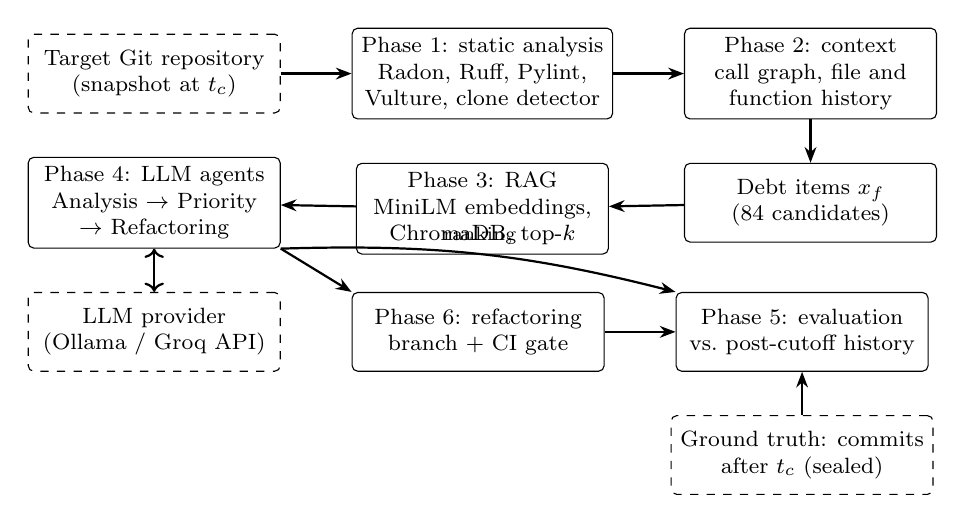
\begin{tikzpicture}[
  box/.style={draw, rounded corners=2pt, align=center, font=\footnotesize, minimum width=3.2cm, minimum height=1.0cm, fill=white},
  ext/.style={box, dashed},
  arr/.style={-{Stealth[length=2mm]}, thick},
  node distance=0.55cm and 0.9cm]
\node[ext] (repo) {Target Git repository\\(snapshot at $t_c$)};
\node[box, right=of repo] (static) {Phase 1: static analysis\\Radon, Ruff, Pylint,\\Vulture, clone detector};
\node[box, right=of static] (ctx) {Phase 2: context\\call graph, file and\\function history};
\node[box, below=of ctx] (items) {Debt items $x_f$\\(84 candidates)};
\node[box, below=of static] (rag) {Phase 3: RAG\\MiniLM embeddings,\\ChromaDB, top-$k$};
\node[box, below=of repo] (agents) {Phase 4: LLM agents\\Analysis $\rightarrow$ Priority\\$\rightarrow$ Refactoring};
\node[ext, below=of agents] (llm) {LLM provider\\(Ollama / Groq API)};
\node[box, right=of llm] (ref) {Phase 6: refactoring\\branch + CI gate};
\node[box, right=of ref] (eval) {Phase 5: evaluation\\vs.\ post-cutoff history};
\node[ext, below=of eval] (truth) {Ground truth: commits\\after $t_c$ (sealed)};
\draw[arr] (repo) -- (static);
\draw[arr] (static) -- (ctx);
\draw[arr] (ctx) -- (items);
\draw[arr] (items) -- (rag);
\draw[arr] (rag) -- (agents);
\draw[arr, <->] (agents) -- (llm);
\draw[arr] (agents.south east) -- (ref.north west);
\draw[arr] (agents.south east) to[bend left=8] node[font=\scriptsize, above]{ranking} (eval.north west);
\draw[arr] (truth) -- (eval);
\draw[arr] (ref) -- (eval);
\end{tikzpicture}
\caption{Architecture of the pipeline. Solid boxes are part of the repository; dashed boxes are external inputs or services. The ground truth is stored in a separate file that no ranking method reads.}
\label{fig:arch}
\end{figure}

As previously stated, the phases in the pipeline save their results as separate files. This was chosen for several reasons. For one, LLM calls can be very slow, and can even fail due to reasons outside of our control (e.g.\ rate limits). In such cases, it is desirable to be able to resume a failed run from the last successfully completed phase. For another, we would like to be able to compare a baseline run to an LLM run on exactly the same set of items. Finally, successful LLM responses are validated against a JSON schema and then cached under a hash of the prompt. This way, we can reproduce a reported run without having to make any further LLM calls.

\subsection{Static and Context Scores}

The composite static score of Phase~1 is a sum of the complexity score, the maintainability score, and a severity bonus that is derived from the Radon rank of the candidate:
\begin{equation}
S(f)=\min\!\left(\frac{CC(f)}{5},\,4\right)+\min\!\left(\max\!\left(0,\frac{100-MI(f)}{25}\right),\,4\right)+b(f),
\label{eq:static}
\end{equation}
with $b(f)=2$ for E and F, $1$ for C and D and $0$ for A and B. $S(f)$ is a number between 0 and 10 and the two caps prevent one metric to dominate the sum.

To test whether an LLM is needed at all, we also define a non-LLM context heuristic. It is the equal-weight mean of min--max normalised features:
\begin{equation}
H(f)=\frac{1}{|\Phi|}\sum_{\phi\in\Phi}\frac{\phi(f)-\min_{g}\phi(g)}{\max_{g}\phi(g)-\min_{g}\phi(g)},
\label{eq:heur}
\end{equation}
where the feature set $\Phi$ consists of $S(f)$, $\log(1+\text{callers})$, the coverage gap $100-\text{coverage}$, and $\log(1+\cdot)$ of function-level commits, function-level fix commits and file-level fix commits, all counted between $t_0$ and $t_c$. A feature that is missing or constant contributes zero. We use logarithms because commit and caller counts are heavily skewed, and equal weights because any fitted weights would have to be learned from labels we want to keep unseen. The ablation ``context without history'' keeps only the first three features.

\subsection{Retrieval and the Agent Chain}

The candidate is rendered as a text document containing location, metrics, findings and history for the candidate. The document is then embedded using the all-MiniLM-L6-v2 Sentence-BERT model \cite{reimers2019} and the $k=5$ most similar items are retrieved from ChromaDB. The neighbours of the candidate are then used to give the model context of how the function compares to other similar debt in the repository. The retrieved items are then frozen to a file, to ensure that every model uses the same context for the candidate.

The next phase of the process, Phase~4, passes the candidate through three agents defined by a role, a goal and a JSON output schema, in the style of multi-agent frameworks \cite{wu2024autogen}. The first of these agents, the Analysis agent, summarises the debt indicators and impact factors for the candidate. The Priority agent then receives this summary and returns a level of HIGH, MEDIUM or LOW, an integer score from 0 to 100 and a reason for the score based on a scoring rubric given in the prompt. The Refactoring agent then returns an action, a refactoring type from a fixed list based on the common catalogue entries for refactoring (e.g.\ Extract Method, Decompose Conditional \cite{fowler2018}) and the expected benefit and the risk for the candidate. The candidates are then sorted by score with ties being broken by level and then by identifier. The work for these three agents is split because asking for analysis, a score and a plan in a single prompt tends to lead to the score not being grounded in the analysis. A single-call mode with a single combined schema is also provided for cheaper comparison runs. The ``without context'' ablation provides only the static metrics and the code for the candidate, with no history and no retrieved neighbours.

\subsection{Refactoring and CI Gate}

For the top $N=5$ items found by Phase~4, Phase~6 asks a refactoring agent for a full replacement of the function, applies the replacement in a separate Git worktree on a branch named \texttt{ai-refactoring/}\emph{function-name}, and runs the target project's test suite. Let $T_0$ be the set of tests that passed on the unmodified snapshot and $T_p$ the set that pass after patch $p$. The patch is accepted only if
\begin{equation}
T_0\subseteq T_p \;\wedge\; CC'(f)<CC(f) \;\wedge\; \mathrm{Ruff}'\le\mathrm{Ruff} \;\wedge\; \mathrm{Dup}'\le\mathrm{Dup},
\label{eq:gate}
\end{equation}
where the prime symbol indicates that the values are measured on the patched file. If the gate fails, then the failing test names and the reason for failure are returned to the model. The model may then try again, up to $R=2$ attempts in total. If a patch changes the function signature or adds unrelated executable statements then the patch is rejected before tests are run. We require a complexity reduction, not only passing tests, because a patch that leaves the function unchanged would otherwise pass trivially.

\subsection{Execution Procedure and Workflow}

Algorithm~\ref{alg:pipeline} provides an overview of the methodology used for the experiments. Fig.~\ref{fig:workflow} shows the time split used for the experiments. All steps prior to the last two steps use the snapshot and history prior to the cutoff, whereas the ground truth for the last step is computed from a separate history window and is read only by the final step.

\begin{algorithm}[!t]
\caption{Time-split debt prioritisation and refactoring}
\label{alg:pipeline}
\KwIn{Repository $G$, dates $t_0<t_c<t_h$, LLM $L$, retrieval size $k$, top $N$, attempts $R$}
\KwOut{Ranking of $\mathcal{F}$, accepted patches, evaluation metrics}
Check out the last commit of $G$ before $t_c$ as snapshot $V$\;
Run the static analysers on $V$; build function index, duplicates and call graph\;
Mine file and function history of $G$ in $[t_0,t_c)$\;
$\mathcal{F}\leftarrow$ functions of $V$ with at least one debt signal; compute $x_f$, $S(f)$, $H(f)$\;
Embed all items; for each $f$ retrieve $\mathcal{N}_k(f)$\;
\ForEach{$f\in\mathcal{F}$}{
  $a\leftarrow L_{\mathrm{analysis}}(x_f,\mathcal{N}_k(f))$\;
  $(\ell_f, s_L(f), r_f)\leftarrow L_{\mathrm{priority}}(x_f, a)$\;
  $\pi_f\leftarrow L_{\mathrm{refactor}}(x_f,a,s_L(f))$\;
}
Sort $\mathcal{F}$ by $s_L$ (ties by level, then identifier)\;
\For{each of the top $N$ functions $f$}{
  \For{$i\leftarrow 1$ \KwTo $R$}{
    Generate patch $p$ on a new branch and run the tests\;
    \lIf{Eq.~(\ref{eq:gate}) holds}{accept $p$ and stop}
    Feed the failures back to $L$\;
  }
}
Compute $y^{\mathrm{fix}}_f, y^{\mathrm{chg}}_f, d_f$ from commits in $[t_c,t_h)$\;
Score every method with Eqs.~(\ref{eq:auc})--(\ref{eq:pk}) and bootstrap intervals\;
\end{algorithm}

\begin{figure}[!t]
\centering
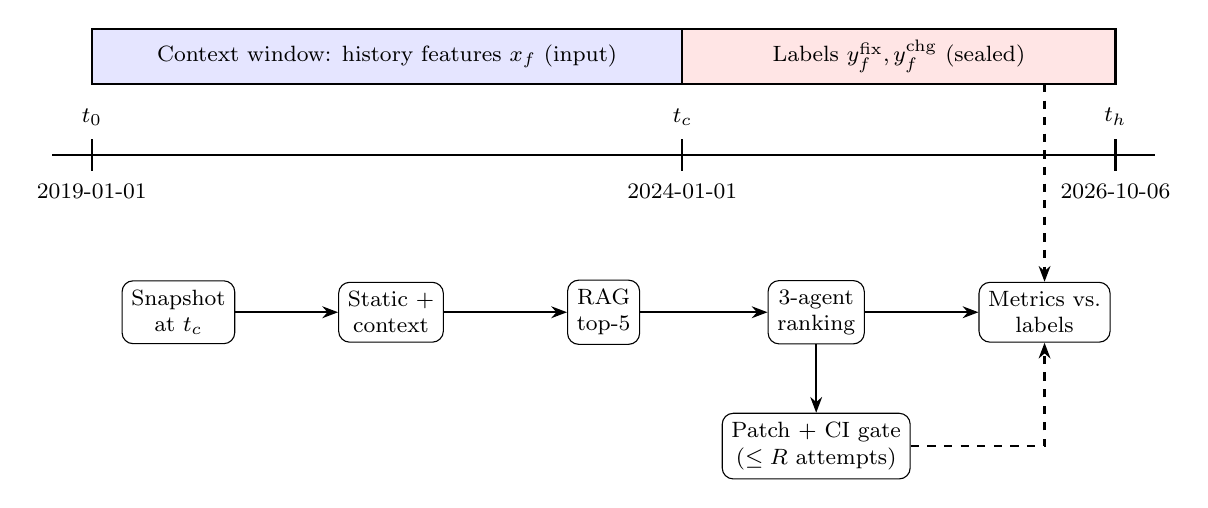
\begin{tikzpicture}[font=\footnotesize, arr/.style={-{Stealth[length=2mm]}, thick}]
\draw[thick] (0,0) -- (14,0);
\foreach \x/\lab/\dt in {0.5/$t_0$/2019-01-01, 8/$t_c$/2024-01-01, 13.5/$t_h$/2026-10-06}{
  \draw[thick] (\x,0.2) -- (\x,-0.2);
  \node[above] at (\x,0.25) {\lab};
  \node[below] at (\x,-0.25) {\dt};}
\draw[thick, fill=blue!10] (0.5,0.9) rectangle (8,1.6);
\node at (4.25,1.25) {Context window: history features $x_f$ (input)};
\draw[thick, fill=red!10] (8,0.9) rectangle (13.5,1.6);
\node at (10.75,1.25) {Labels $y^{\mathrm{fix}}_f, y^{\mathrm{chg}}_f$ (sealed)};
\node[draw, rounded corners, fill=white, align=center] (s1) at (1.6,-2.0) {Snapshot\\at $t_c$};
\node[draw, rounded corners, fill=white, align=center] (s2) at (4.3,-2.0) {Static +\\context};
\node[draw, rounded corners, fill=white, align=center] (s3) at (7.0,-2.0) {RAG\\top-5};
\node[draw, rounded corners, fill=white, align=center] (s4) at (9.7,-2.0) {3-agent\\ranking};
\node[draw, rounded corners, fill=white, align=center] (s5) at (12.6,-2.0) {Metrics vs.\\labels};
\node[draw, rounded corners, fill=white, align=center] (s6) at (9.7,-3.7) {Patch + CI gate\\($\le R$ attempts)};
\draw[arr] (s1) -- (s2); \draw[arr] (s2) -- (s3); \draw[arr] (s3) -- (s4); \draw[arr] (s4) -- (s5);
\draw[arr] (s4) -- (s6); \draw[arr, dashed] (s6.east) -| (s5.south);
\draw[arr, dashed] (12.6,0.9) -- (s5.north);
\end{tikzpicture}
\caption{Workflow and time split. Inputs (blue) come only from history before the cutoff $t_c$; labels (red) come only from commits after it and enter the pipeline at the final evaluation step.}
\label{fig:workflow}
\end{figure}

\subsection{Evaluation Measures}

Each method $M$ is judged as a ranker. We use Spearman's $\rho$ between the method's scores and the number of later changes to measure agreement with how often functions change, and the area under the ROC curve for the defect label,
\begin{equation}
\mathrm{AUC}_M=\frac{1}{|P||N|}\sum_{i\in P}\sum_{j\in N}\left(\mathbf{1}[s_M(i)>s_M(j)]+\tfrac{1}{2}\mathbf{1}[s_M(i)=s_M(j)]\right),
\label{eq:auc}
\end{equation}
The functions with $d_f=1$ are counted as $P$ and the functions with $d_f=0$ are counted as $N$. Ties are counted as 0.5. Since the developers mainly focus on the top of a list of functions, we also compute the normalized discounted cumulative gain \cite{jarvelin2002} with graded gain $y^{\mathrm{fix}}$.
\begin{equation}
\mathrm{NDCG@}K=\frac{\sum_{r=1}^{K} y^{\mathrm{fix}}_{(r)}/\log_2(r+1)}{\sum_{r=1}^{K} y^{\mathrm{fix}}_{[r]}/\log_2(r+1)},
\label{eq:ndcg}
\end{equation}
where $(r)$ is the item at position $r$ of the method's ranking, and $[r]$ is the item at position $r$ of the ideal ranking, for each of the $K$ positions, and the precision at $K$.
\begin{equation}
\mathrm{P@}K=\frac{|\{f\in\text{top-}K(s_M): d_f=1\}|}{K}.
\label{eq:pk}
\end{equation}
Differences between two methods are tested with a paired bootstrap \cite{efron1993} of $\Delta\rho$ on the same items, and a difference is called significant when its 95\% interval excludes zero.

\section{Experimental Setup}
\label{sec:setup}

\textbf{Dataset.} The Requests library was used as the source package for this experiment. This widely used Python HTTP client has a long, public history. The snapshot used for this experiment was commit \texttt{72eccc8d}, the last commit before 1 January 2024. The context history starts on 1 January 2019 and the ground-truth window ends on 6 October 2026. The source package consists of 18 files, 5,426 physical lines of code and 235 functions. The analysers reported 500 findings (Radon 53, Ruff 110, Pylint 281, Vulture 56) and 84 functions met the candidate rule. After the cutoff date, 28 of the 84 candidates were changed and 7 received at least one bug-fix commit. A commit is considered a bug fix if its message contains words such as ``fix'', ``bug'', ``error'' or ``regression'' and the subject does not contain the word ``typos'', ``documentation'', ``CI'', ``typing'' or ``release''. Commits that touch more than 25 functions (e.g.\ reformatting passes) are ignored. Coverage was not attached to this snapshot so the coverage feature is constant and contributes nothing to the score. There is no training split so no method was fitted to the labels.

\textbf{Tools.} The pipeline was run with Python 3.11 using Radon 6.0.1, Ruff 0.16.10, Pylint 4.1.2, Vulture 2.16, GitPython 3.1.45, ChromaDB 1.5.5, sentence-transformers 5.3.0, SciPy 1.16.1 and pytest 9.0.2 on a Windows 11 laptop with 18 logical CPUs and 15.8 GB of RAM. The full-dataset LLM run was done using SmolLM2 with 1.7 billion parameters \cite{allal2025smollm2} running locally via Ollama with a temperature of 0. Paid API credit was not available at the time of the experiment. A seeded 30-item pilot was run with two open-weight GPT-OSS models (20B and 120B) via the Groq API in single-call mode.

\textbf{Baselines.} We compare five rankers: the composite static score $S(f)$, raw cyclomatic complexity, the context heuristic $H(f)$, the context heuristic without history features, and the proposed LLM with RAG context. Complexity is the most common prioritisation rule in practice, and the heuristics test whether repository context helps without a language model.

\textbf{Metrics.} Spearman's $\rho$ with future changes measures overall agreement with maintenance effort; ROC-AUC measures whether bug-fixed functions are ranked above clean ones regardless of a threshold; NDCG@10 and P@5/P@10 measure the quality of the short list a developer would actually read. For refactoring we report the gate pass rate, new test failures and the change in complexity.

\textbf{Repetitions.} The non-LLM rankers are deterministic. For the SmolLM2 run with temperature 0 we use cached responses. Thus, a rerun on the same items would yield the same ranking. We therefore report the uncertainty as the standard deviation of 1,000 bootstrap resamples of the items. This captures the main source of variation, which functions are in the sample. In addition, the 30-item pilot was repeated three times with SmolLM2, with and without RAG context, with the response cache turned off. All settings are listed in Table~\ref{tab:params}.

\begin{table}[!t]
\centering
\caption{Experimental Parameters}
\label{tab:params}
\small
\fitwidth{\begin{tabular}{lll}
\toprule
\textbf{Group} & \textbf{Parameter} & \textbf{Value} \\
\midrule
\multirow{5}{*}{Dataset} & Snapshot / cutoff $t_c$ & \texttt{72eccc8d} / 2024-01-01 \\
 & Context start $t_0$ / horizon $t_h$ & 2019-01-01 / 2026-10-06 \\
 & Candidate rule & $CC\ge6$, smell, dead code, dup $\ge6$ or LOC $\ge60$ \\
 & Candidates / changed / bug-fixed & 84 / 28 / 7 \\
 & Sweeping-commit limit & 25 functions per commit \\
\midrule
\multirow{4}{*}{RAG} & Embedding model & all-MiniLM-L6-v2 \\
 & Vector store & ChromaDB, batch size 64 \\
 & Neighbours $k$ & 5 \\
 & Neighbours checked & 70 queries, 5 each, no self-matches \\
\midrule
\multirow{5}{*}{LLM} & Full-run model & SmolLM2 1.7B (Ollama, Q8\_0), $T=0$ \\
 & Pilot models & GPT-OSS 20B and 120B (Groq) \\
 & Agent mode & 3-agent chain (full run); single call (pilot) \\
 & Max output tokens & 2,048 \\
 & Pilot sample / repeats & 30 items, seed 7 / 1 (GPT-OSS), 3 (SmolLM2) \\
\midrule
\multirow{2}{*}{Refactoring} & Top $N$ / attempts $R$ & 5 / 2 \\
 & Baseline test run & 591 passed, 2 failed (pre-existing) \\
\midrule
Statistics & Bootstrap resamples & 1,000 (SD); 2,000 (paired $\Delta\rho$), seed 42 \\
\bottomrule
\end{tabular}}
\end{table}

\section{Results and Analysis}
\label{sec:results}

\subsection{RQ1: Ranking Quality against Post-Cutoff History}

SmolLM2 chain returned a valid ranking for 71 of the 84 candidates, 13 were cut off before completion. All methods can be compared on the 71 functions for which a valid ranking was returned by SmolLM2 chain. Note that 5 of these 71 functions were bug-fixed after the cutoff. The LLM ranking is the weakest on all metrics (Table~\ref{tab:main}). The correlation with future changes is 0.139 (vs.\ 0.507 for raw complexity) and the AUC is 0.494 (close to random order). The context heuristic is best on AUC, NDCG@10 and P@5 while the complexity is best on correlation with change counts.

\begin{table}[!t]
\centering
\caption{Ranking Quality on 71 Functions (Point Estimate $\pm$ Bootstrap SD, 1,000 Resamples; Best in Bold)}
\label{tab:main}
\footnotesize
\setlength{\tabcolsep}{4pt}
\fitwidth{\begin{tabular}{lccccc}
\toprule
\textbf{Method} & $\boldsymbol{\rho}$ \textbf{(changes)} & \textbf{AUC (defect)} & \textbf{NDCG@10} & \textbf{P@5} & \textbf{P@10} \\
\midrule
Static composite $S(f)$ & 0.413 $\pm$ 0.107 & 0.815 $\pm$ 0.114 & 0.468 $\pm$ 0.181 & 0.20 $\pm$ 0.22 & \textbf{0.30} $\pm$ 0.16 \\
Complexity only & \textbf{0.507} $\pm$ 0.090 & 0.811 $\pm$ 0.103 & 0.611 $\pm$ 0.233 & 0.40 $\pm$ 0.22 & \textbf{0.30} $\pm$ 0.15 \\
Context, no history & 0.363 $\pm$ 0.103 & 0.879 $\pm$ 0.050 & 0.401 $\pm$ 0.216 & 0.40 $\pm$ 0.21 & 0.20 $\pm$ 0.14 \\
Context heuristic $H(f)$ & 0.424 $\pm$ 0.100 & \textbf{0.912} $\pm$ 0.053 & \textbf{0.667} $\pm$ 0.240 & \textbf{0.60} $\pm$ 0.25 & \textbf{0.30} $\pm$ 0.17 \\
LLM + RAG (SmolLM2) & 0.139 $\pm$ 0.118 & 0.494 $\pm$ 0.142 & 0.076 $\pm$ 0.104 & 0.20 $\pm$ 0.12 & 0.10 $\pm$ 0.08 \\
\bottomrule
\end{tabular}}
\end{table}

The three LLM ranking metrics in Fig.~\ref{fig:bars} are lower than the corresponding metrics for the other four methods. The whiskers for the four non-LLM methods overlap widely because there are only five bug-fixed functions, and moving one of them by a few places would result in a change in NDCG@10 of more than 0.1.

\begin{figure}[!t]
\centering
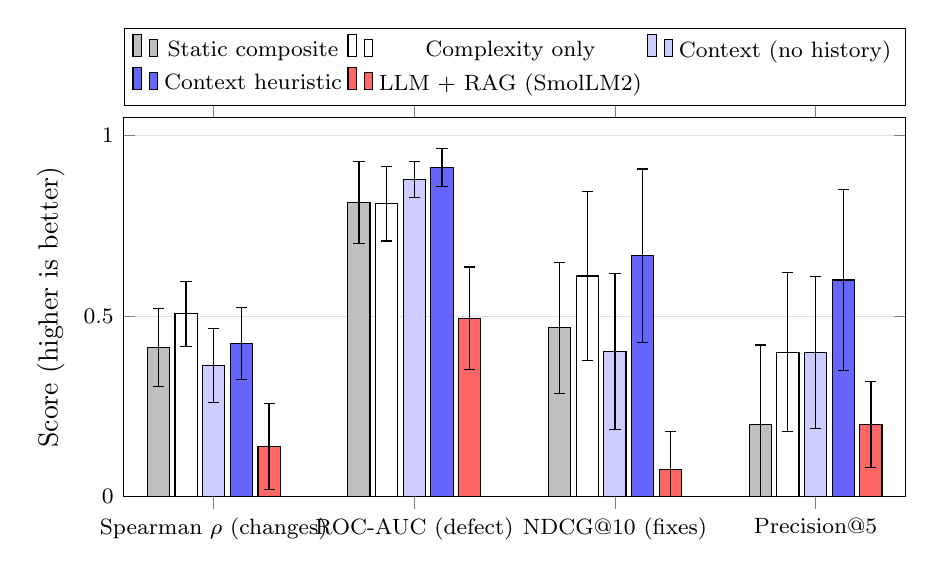
\begin{tikzpicture}
\begin{axis}[
  ybar, width=0.95\textwidth, height=6.4cm, bar width=8pt,
  ymin=0, ymax=1.05, ylabel={Score (higher is better)},
  symbolic x coords={rho,AUC,NDCG,P5}, xtick=data,
  xticklabels={Spearman $\rho$ (changes), ROC-AUC (defect), NDCG@10 (fixes), Precision@5},
  legend style={at={(0.5,1.03)}, anchor=south, legend columns=3, font=\footnotesize},
  error bars/y dir=both, error bars/y explicit,
  ymajorgrids, grid style={gray!25}, enlarge x limits=0.15, tick label style={font=\footnotesize}]
\addplot[fill=gray!50] coordinates {(rho,0.413) +- (0,0.107) (AUC,0.815) +- (0,0.114) (NDCG,0.468) +- (0,0.181) (P5,0.20) +- (0,0.22)};
\addplot[fill=white] coordinates {(rho,0.507) +- (0,0.090) (AUC,0.811) +- (0,0.103) (NDCG,0.611) +- (0,0.233) (P5,0.40) +- (0,0.22)};
\addplot[fill=blue!20] coordinates {(rho,0.363) +- (0,0.103) (AUC,0.879) +- (0,0.050) (NDCG,0.401) +- (0,0.216) (P5,0.40) +- (0,0.21)};
\addplot[fill=blue!60] coordinates {(rho,0.424) +- (0,0.100) (AUC,0.912) +- (0,0.053) (NDCG,0.667) +- (0,0.240) (P5,0.60) +- (0,0.25)};
\addplot[fill=red!60] coordinates {(rho,0.139) +- (0,0.118) (AUC,0.494) +- (0,0.142) (NDCG,0.076) +- (0,0.104) (P5,0.20) +- (0,0.12)};
\legend{Static composite, Complexity only, Context (no history), Context heuristic, LLM + RAG (SmolLM2)}
\end{axis}
\end{tikzpicture}
\caption{Ranking quality of the five methods on 71 functions. Bars are point estimates and whiskers are $\pm$1 bootstrap standard deviation (1,000 item resamples).}
\label{fig:bars}
\end{figure}

The comparison of shared items between the methods is presented in Table~\ref{tab:paired}. Only the difference between LLM and complexity is significantly negative ($\Delta\rho=-0.369$). The confidence intervals for the comparisons with static score and context heuristic end slightly above zero. The LLM is not better than any method.

\begin{table}[!t]
\centering
\caption{Paired Bootstrap Differences in Spearman $\rho$ against Future Changes}
\label{tab:paired}
\small
\fitwidth{\begin{tabular}{lcccc}
\toprule
\textbf{Comparison} & \textbf{Items} & $\boldsymbol{\Delta\rho}$ & \textbf{95\% CI} & \textbf{Significant} \\
\midrule
LLM $-$ static composite & 71 & $-$0.275 & [$-$0.570, 0.035] & no \\
LLM $-$ complexity & 71 & $-$0.369 & [$-$0.637, $-$0.070] & \textbf{yes} \\
LLM $-$ context heuristic & 71 & $-$0.285 & [$-$0.551, 0.005] & no \\
Context heuristic $-$ no history & 84 & +0.050 & [$-$0.162, 0.260] & no \\
Advanced history $-$ context heuristic & 84 & $-$0.157 & [$-$0.256, $-$0.067] & \textbf{yes} \\
\bottomrule
\end{tabular}}
\end{table}

Fig.~\ref{fig:scores} shows why the ranking is weak. Although the rubric for the ranking task specified the entire 0--100 range, the model used 11 distinct values and scored 44 of the 71 functions with 2, 20 or 80. The 5 functions that were later bug-fixed were scored 80, 50, 20, 6 and 2. For example, \texttt{Session.request} was scored 20. The written reasons for the scores are plausible but the numeric scores do not follow the reasons consistently.

\begin{figure}[!t]
\centering
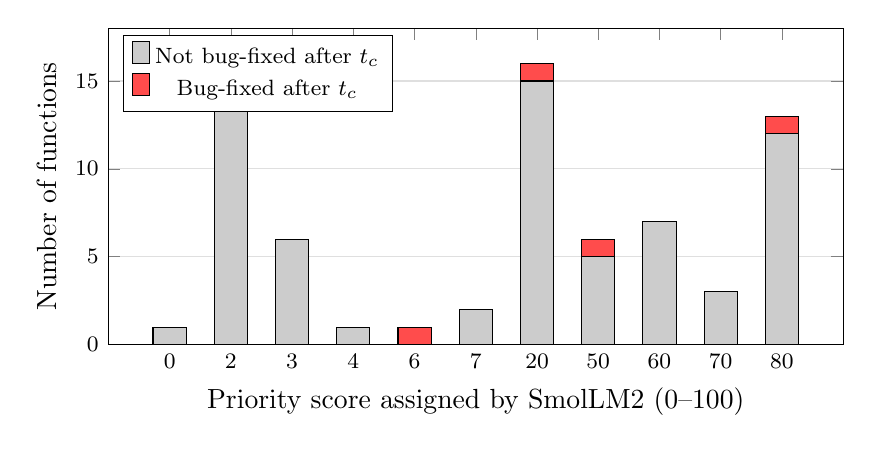
\begin{tikzpicture}
\begin{axis}[
  ybar stacked, width=0.9\textwidth, height=5.6cm, bar width=12pt,
  ymin=0, ymax=18, ylabel={Number of functions}, xlabel={Priority score assigned by SmolLM2 (0--100)},
  symbolic x coords={0,2,3,4,6,7,20,50,60,70,80}, xtick=data,
  legend style={at={(0.02,0.98)}, anchor=north west, font=\footnotesize},
  ymajorgrids, grid style={gray!25}, tick label style={font=\footnotesize}]
\addplot[fill=gray!40] coordinates {(0,1) (2,14) (3,6) (4,1) (6,0) (7,2) (20,15) (50,5) (60,7) (70,3) (80,12)};
\addplot[fill=red!70] coordinates {(0,0) (2,1) (3,0) (4,0) (6,1) (7,0) (20,1) (50,1) (60,0) (70,0) (80,1)};
\legend{Not bug-fixed after $t_c$, Bug-fixed after $t_c$}
\end{axis}
\end{tikzpicture}
\caption{Distribution of the priority scores given by the LLM chain to the 71 ranked functions. Only 11 distinct scores were used, and the five later bug-fixed functions are spread across the scale.}
\label{fig:scores}
\end{figure}

\subsection{Model Size and Context Ablation}

To understand if the results we obtained for the small model are also valid for larger models we run two of the GPT-OSS models on the seeded 30-item sample with three bug-fixed functions. In Table~\ref{tab:pilot} we compare the results of each run with the results of the baselines on the same items. For the larger models the results are indeed better than for the SmolLM2 model (20B: AUC 0.925, NDCG@10 0.900), however on the same items for the larger models the complexity measure reaches an AUC of 1.000 and the context heuristic reaches an NDCG@10 of 0.954, so no LLM run is able to outperform the best baseline on any of the metrics. For the 20B model 7 of the 30 items could not be evaluated without context and for all 30 items with RAG context the provider rate limits were exceeded.

\begin{table}[!t]
\centering
\caption{Pilot on a Seeded 30-Item Sample: LLMs and Baselines on the Same Items (Best per Item Set in Bold)}
\label{tab:pilot}
\footnotesize
\setlength{\tabcolsep}{4pt}
\fitwidth{\begin{tabular}{llcccccc}
\toprule
\textbf{Item set} & \textbf{Method} & $\boldsymbol{\rho}$ & \textbf{AUC} & \textbf{NDCG@10} & \textbf{Time (s)} & \textbf{Cost (USD)} & \textbf{Failed} \\
\midrule
\multirow{5}{*}{23 shared} & GPT-OSS 20B, no context & 0.421 & 0.925 & 0.900 & 154.6 & 0.0039 & 7/30 \\
 & GPT-OSS 120B, no context & 0.243 & 0.900 & 0.590 & 172.0 & 0.0094 & 0/30 \\
 & Static composite & 0.583 & \textbf{1.000} & 0.840 & -- & -- & -- \\
 & Complexity only & \textbf{0.612} & \textbf{1.000} & 0.882 & -- & -- & -- \\
 & Context heuristic & 0.443 & 0.950 & \textbf{0.954} & -- & -- & -- \\
\midrule
\multirow{5}{*}{All 30} & GPT-OSS 120B, no context & 0.337 & 0.895 & 0.555 & 172.0 & 0.0094 & 0/30 \\
 & GPT-OSS 120B, RAG context & 0.451 & 0.889 & 0.853 & 447.1 & 0.0148 & 0/30 \\
 & Static composite & 0.561 & \textbf{1.000} & 0.840 & -- & -- & -- \\
 & Complexity only & \textbf{0.608} & \textbf{1.000} & 0.882 & -- & -- & -- \\
 & Context heuristic & 0.486 & 0.926 & \textbf{0.936} & -- & -- & -- \\
\bottomrule
\end{tabular}}
\end{table}

For the 120B model on the 30-item sample both arms of the matched ablation were completed. The addition of RAG context resulted in an increase of $\rho$ from 0.337 to 0.451 and an increase of NDCG@10 from 0.555 to 0.853. The AUC remained almost unchanged. The context helped the larger model to rank frequently changed and bug-fixed functions higher. However, the run time increased by a factor of 2.6 and the token cost increased by a factor of 1.6. Since only three positive examples and one run were used in the evaluation the effect can only be suggested but not established.

Table~\ref{tab:repeats} shows three repeats of SmolLM2 in single-call mode on the same 30 items, with and without RAG context. Both arms stay close to random order (AUC 0.454 and 0.532), so the weak result in Table~\ref{tab:main} is not caused by one unlucky run. The RAG repeats gave identical scores because the temperature is 0. The small spread in the no-context arm comes from one item that timed out in two of the three runs. In single-call mode the model used only three or four distinct scores, which makes the score collapse in Fig.~\ref{fig:scores} even stronger.

\begin{table}[!t]
\centering
\caption{SmolLM2 on the 30-Item Pilot, Single-Call Mode (Mean $\pm$ SD over 3 Repeats)}
\label{tab:repeats}
\small
\fitwidth{\begin{tabular}{lcccc}
\toprule
\textbf{Arm} & $\boldsymbol{\rho}$ \textbf{(changes)} & \textbf{AUC} & \textbf{NDCG@10} & \textbf{Item failures} \\
\midrule
No context  & \textbf{0.201} $\pm$ 0.050 & 0.454 $\pm$ 0.010 & \textbf{0.241} $\pm$ 0.011 & 5.6\% $\pm$ 1.9\% \\
RAG context & 0.160 $\pm$ 0.000 & \textbf{0.532} $\pm$ 0.000 & 0.202 $\pm$ 0.000 & \textbf{3.3\%} $\pm$ 0.0\% \\
\bottomrule
\end{tabular}}
\end{table}

\subsection{Git-History Ablation}

The context heuristic provides us with the value of the history features without the LLM. Dropping the three history features led to a defect AUC of 0.879 and NDCG@10 of 0.401 for the 71 items in Table~\ref{tab:main}. For all 84 items, dropping the history features led to a drop of $\rho$ by 0.050, although that is within the interval that includes zero for that metric in Table~\ref{tab:paired}. Thus, the most useful signal for placing future fixes near the top of the list of functions to fix is past fixes in a function. On the other hand, adding more history features (churn, number of authors, recency and a recurring-bug flag) with equal weight led to a significant drop of $\rho$ by 0.157. Thus, more history is not necessarily better: unweighted features that are only loosely related to future changes dilute the useful features.

\subsection{RQ2: Refactoring through the CI Gate}

Table~\ref{tab:refactor} lists the five attempts at refactoring the top-ranked functions. None of the five attempts at refactoring the top-ranked functions passed the gate. For the function \texttt{RequestsCookieJar.update} the model produced invalid JSON, for \texttt{cookiejar\_from\_dict} both attempts were rejected by the safety checks, first for adding a public helper and then for adding code outside the target function. For \texttt{api.patch} the patch kept all 593 tests passing and removed 8 duplicated lines, but it was rejected because the complexity of a function that already had complexity 1 could not be reduced any further. For \texttt{PreparedRequest.prepare\_body} the patch reduced complexity from 17 to 15 but failed on 15 tests for chunked uploads and body rewinding. For \texttt{HTTPDigestAuth.handle\_401} the patch failed on 8 tests for digest-authentication. The mean number of attempts was 1.8 and the mean complexity reduction over the applied patches was 0.67.

\begin{table}[!t]
\centering
\caption{LLM Refactoring Attempts and CI Gate Outcome (SmolLM2, Top 5 Functions)}
\label{tab:refactor}
\small
\fitwidth{\begin{tabular}{lcccl}
\toprule
\textbf{Function} & \textbf{CC before $\rightarrow$ after} & \textbf{Tests passed} & \textbf{New failures} & \textbf{Gate result} \\
\midrule
\texttt{api.patch} & 1 $\rightarrow$ 1 & 593 & 0 & Rejected (no CC reduction) \\
\texttt{HTTPDigestAuth.handle\_401} & 5 $\rightarrow$ 5 & 585 & 8 & Rejected (tests) \\
\texttt{RequestsCookieJar.update} & 3 $\rightarrow$ -- & -- & -- & No applicable patch \\
\texttt{cookiejar\_from\_dict} & 7 $\rightarrow$ -- & -- & -- & No applicable patch \\
\texttt{PreparedRequest.prepare\_body} & 17 $\rightarrow$ 15 & 578 & 15 & Rejected (tests, Ruff +1) \\
\midrule
\textbf{Total} & mean $-$0.67 & -- & -- & \textbf{0/5 accepted} \\
\bottomrule
\end{tabular}}
\end{table}

A poor ranking in the previous step also led to bad results in the next step. As can be seen from Table~\ref{tab:refactor}, three of the five ``top'' functions had complexity of 5 or less. This did not leave much room for improvement. The gate blocked all behavior-changing patches and even gave feedback on which behavior was broken by the patch.

\subsection{Runtime Cost}

Fig.~\ref{fig:scale}: Non-LLM stages on synthetic repositories of 0.5, 5 and 25 thousand lines. The structural analysis and the static analysis are very fast ($<$3\,s and $<$6\,s, respectively). The RAG indexing, however, takes more time (up to 120\,s) and even more memory (up to 695\,MB, mostly used by the embedding model). On Requests, the history mining takes 13.0 of the 13.8 seconds of context building. All of these stages are very small compared to the LLM (154--447\,s for 30 items).

\begin{figure}[!t]
\centering
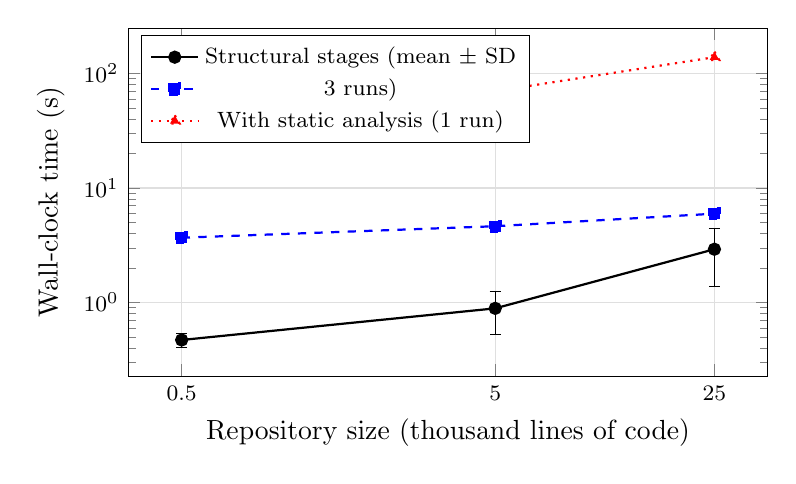
\begin{tikzpicture}
\begin{loglogaxis}[
  width=0.8\textwidth, height=6cm,
  xlabel={Repository size (thousand lines of code)}, ylabel={Wall-clock time (s)},
  xtick={0.495,4.95,24.75}, xticklabels={0.5,5,25},
  legend style={at={(0.02,0.98)}, anchor=north west, font=\footnotesize},
  grid=major, grid style={gray!25}, tick label style={font=\footnotesize},
  error bars/y dir=both, error bars/y explicit]
\addplot[mark=*, thick, black] coordinates {(0.495,0.470) +- (0,0.063) (4.95,0.888) +- (0,0.361) (24.75,2.917) +- (0,1.532)};
\addplot[mark=square*, thick, blue, dashed] coordinates {(0.495,3.677) (4.95,4.634) (24.75,5.963)};
\addplot[mark=triangle*, thick, red, dotted] coordinates {(0.495,48.72) (4.95,70.13) (24.75,138.82)};
\legend{Structural stages (mean $\pm$ SD, 3 runs), With static analysis (1 run), With RAG indexing (1 run)}
\end{loglogaxis}
\end{tikzpicture}
\caption{Wall-clock time of the non-LLM pipeline stages against repository size on synthetic fixtures. Both axes are logarithmic.}
\label{fig:scale}
\end{figure}

In summary, for RQ1, the answer is negative for the model we can run on the full dataset, and not yet positive for larger models: no LLM ranking can beat raw complexity or the context heuristic. For RQ2, the answer is negative as well: no generated refactoring can pass the gate, but the gate can block all harmful patches.

\section{Discussion}
\label{sec:discussion}

These results primarily speak to the baselines. A simple one-line rule, sort by cyclomatic complexity, and a simple equal-weight mix of six pre-cutoff features are hard to beat. This is consistent with the findings of defect-prediction research that found process metrics to carry most of the signal for defect-prediction \cite{nagappan2005,kamei2013}. For a team choosing a tool, the practical message is that an LLM prioritiser should be reported next to such baselines, on the same items, under a time split; a ranking that only looks sensible in its written reasons can still be no better than random, as the AUC of 0.494 shows.

The LLM struggled for two main reasons. First, the small model that we were able to run on the full dataset compressed the scores into a small number of values, and so the ranking had very low resolution. Simple remedies include asking for pairwise comparisons, or for a calibrated scale, or for the LLM score to be combined with the heuristic score. Second, the model had to infer risk from the same numbers that the heuristic uses directly; with the history already in the prompt, the model's language ability adds little unless it can read signals that numbers miss, such as an unclear interface. The 120B ablation suggests that the retrieved context can help a capable model, but the gain is small next to the strong baselines.

There are several limitations to this work. For instance, the study only uses one mature repository and one snapshot of it with only five to seven bug-fixed functions. The full-dataset experiment was run with a 1.7B model because we ran out of paid API credit. The larger models were only tested on 30 items once. No coverage was measured and no human expert ratings were collected. Thus, the term ``priority'' in this study is only measured through later fixes and changes.

\textbf{Threats to validity.} We use commit messages to identify bug fixes. However, there are silent bug fixes and some bug fixes are mislabeled as other types of changes \cite{sliwerski2005}. Future changes are used as a proxy for debt urgency, but they do not measure debt urgency directly. The models may have been trained on the public code of Requests, which may give the LLM an advantage over the non-LLM baselines. In addition, function renames after the cutoff may hide some changes. When we audited the results of the LLM rankings on the working directory, we found that one of the saved copies of the LLM rankings had scores that did not match the model's cached responses. We discarded that file and recomputed all of the LLM results in this paper from the cached raw responses, which reproduce the originally generated evaluation report exactly. \textbf{Ethics.} We only analyzed the public open-source code of Requests. We did not push any patches to the upstream project. No personal data was used.

\section{Conclusion and Future Work}
\label{sec:conclusion}

In this work we evaluate a pipeline for technical debt prioritization and refactoring using static analysis, repository history and RAG. The evaluation is conducted on the Requests library using a strict time split. For RQ1, the LLM-based ranking did not outperform static analysis and the simple context heuristic. The SmolLM2 chain achieved a Spearman correlation of 0.139 and a defect AUC of 0.494 on 71 functions, whereas complexity scored 0.507 and the context heuristic scored an AUC of 0.912. For the larger GPT-OSS models the gap to the best baselines is narrowed but not closed. For RQ2, none of the 5 generated refactorings passed the CI gate. However, the gate did successfully block all behavior-changing patches. The function-level fix history was found to be the most useful context signal. Adding more history features, with equal weight, actually hurt the ranking.

There are three main directions for future work. First, the full 84-item experiment should be repeated with larger models over several seeds, together with the matched no-context arm, so that the 120B context gain can be tested with proper statistics. Second, the LLM should be used as a re-ranker of the context heuristic's top items, or asked for pairwise judgements, to avoid the score collapse seen here. Third, the study should be extended to several repositories with measured coverage and to blind ratings from at least two independent developers, so that the ground truth reflects expert judgement as well as history.

\section*{Code Repository and Reproducibility}

The source code, saved datasets, cached LLM responses and evaluation scripts are available at \url{https://github.com/sahil45-ops/Ai-dev-project}. Running \texttt{python run\_evaluation.py} reproduces Tables~\ref{tab:main} and~\ref{tab:paired} from the cached responses, and \texttt{run\_model\_benchmark.py} and \texttt{run\_scalability.py} reproduce the pilot and runtime results.

\section*{AI-Use Declaration}

An AI assistant (Claude, Anthropic) was used to audit the saved experiment files, recompute metrics from the cached model responses, run the repeated SmolLM2 experiment, and draft the text and figures of this paper. The authors checked every number against the experiment outputs, read the cited sources, and revised the text in their own words.

\section*{Author Contributions}

\noindent Sahil Mahadev Mane (230545): system design, static analysis and repository-context phases, time-split dataset construction, LLM agent chain and RAG retrieval, evaluation framework, and writing of the paper.\\
Asad Ahmad (230516): refactoring CI gate and branch validation, model benchmark and scalability experiments, dashboard and live analysis server, CI workflow and Docker deployment, and figures and results analysis.\\
Ayush Singh (230556): literature collection for related work and proofreading of the paper.\\
Naveen Singh/Kiran Khatter: supervision and review.

\bibliographystyle{IEEEtran}
\bibliography{references}

\end{document}
